\section{Rules, Values and Conventions}\label{sec:rules}

\subsection{The Board and the Moves}
We play ordinary chess on the \emph{cylinder}, the $8\times8$ board with the a-file joined to the h-file. Only
the files wrap: ranks 1 and 8 are still edges. Every piece may cross the seam: a white pawn on h4 can capture on
a5, a knight on h1 gains a3 and b2, and a king on h1 gains a1 and a2, so a checkmate on the ordinary board need
not be one on the cylinder. A sliding piece stops before its ray returns to its own square, so a rook cannot
circle a rank as a null move. En passant (e.p.) is allowed, across the seam too. We write $\cyl{n}$ and
$\flatb{n}$ for the cylinder and the ordinary board with $n$ files and eight ranks.

\subsection{Notation}\label{sec:notation}
We write $G=\game{G^L}{G^R}$ when white (Left) can move to the positions $G^L$ and black (Right) to $G^R$, and
$G+H$ for the sum in which the player to move chooses one component~\cite{WinningWays,ONAG,Siegel2013}. Every
finite game has a unique \emph{canonical form}, obtained by deleting dominated options and bypassing reversible
ones, and $G=H$ exactly when $G-H$ is a second-player win. The \emph{outcome class} of $G$ is $\mathcal{L}$ if
white wins whoever starts, $\mathcal{R}$ if black does, $\mathcal{N}$ if the first player wins and
$\mathcal{P}$ if the second does. Our values include \emph{numbers} (integers and dyadic fractions such as
$1/2=\game{0}{1}$), \emph{nimbers} $\nim{k}$ (Section~\ref{sec:intro}), and \emph{switches} $\pm x=\game{x}{-x}$ with $x>0$. Sums are written without the plus sign,
so for a number $a$, $a\pm x=a+(\pm x)=\game{a+x}{a-x}$. The \emph{birthday} of a game is the height of its
canonical game tree, so $\nim{k}$ has birthday $k$. Each game has a \emph{mean} and a \emph{temperature}, read
from its thermograph~\cite{WinningWays}; $\pm x$ has mean $0$ and temperature $x$. The \emph{left} and
\emph{right stops} of $G$ are the numbers reached when white or black moves first and both sides play until a
number appears; both stops of $0$ and of $\nim{2}$ are $0$. Infinitesimals such as ${\uparrow}=\game{0}{\star}$ and
$\tinyg{1}=\ggame{0}{0\mid -1}$ are introduced with their positions in Section~\ref{sec:basic}.

\subsection{Normal Play and the Passed-Pawn Convention}
Following Elkies~\cite{Elkies1996}, we change chess just enough to fit normal play~\cite{WinningWays}.
\begin{itemize}
\item In pawn-only positions, a player who has no move loses; there are no null moves.
\item A position in which exactly one side has a passed pawn is decided, worth $+\BIG$ if that pawn is white and
  $-\BIG$ if it is black, where $\BIG$ exceeds any count of spare moves (our programs use $\BIG=256$).
\item Kings are added as a group in mutual zugzwang, the tr\'ebuchet, and are then \emph{frozen}: the model
  never moves them and counts the group as $0$, since whoever moves a king there first loses a pawn, and then
  the game. Section~\ref{sec:kings} asks when this is exact.
\end{itemize}
A move, usually a capture, can give both sides a passed pawn; such a race needs a rule:
\begin{itemize}
\item \emph{count}: fewer moves to promote wins; the side that did not move goes first and wins a tie;
\item \emph{mover}: the side that made the move wins;
\item \emph{opponent}: the other side wins.
\end{itemize}
None is exact chess, since a new queen may give check or stop the other pawn.

\subsection{En Passant and the Passed-Pawn Test}\label{sec:ep}
The textbook test calls a pawn passed if no enemy pawn stands ahead of it on its own file or a neighboring file
(on the cylinder, a and h are neighbors). En passant breaks this test: after a2--a4 in Fig.~\ref{fig:ep_test}
the textbook test calls the a-pawn passed, yet black takes it en passant, b4$\times$a3. Elkies asked for a
more systematic treatment of en passant~\cite{Elkies1996}; we use a stricter test.

\begin{figure}[!t]
\centering
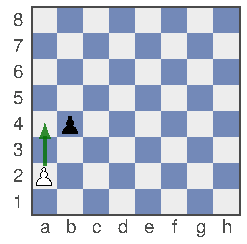
\includegraphics[width=0.36\columnwidth]{figures/ep_test.pdf}
\caption{Position \pos{W a2 / B b4} (ordinary board), value $0$. After a2--a4 (arrow) the textbook test calls the
a-pawn passed, but b4$\times$a3 en passant removes it; under Definition~\ref{def:epaware} it is not passed.}
\label{fig:ep_test}
\end{figure}

% Fig. 2 belongs to Section III; it is defined here so that the full-width float lands next to it.
\begin{figure*}[!t]
\centering
\begin{subfigure}[t]{0.16\textwidth}\centering
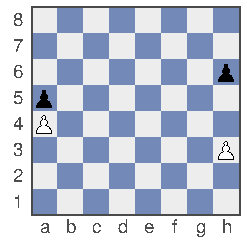
\includegraphics[width=\linewidth]{figures/zero_seam.pdf}
\caption{\pos{W~a4~h3 / B~a5~h6}: $0$}
\end{subfigure}\hfill
\begin{subfigure}[t]{0.16\textwidth}\centering
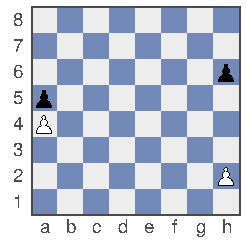
\includegraphics[width=\linewidth]{figures/one.pdf}
\caption{\pos{W~a4~h2 / B~a5~h6}: $1$}
\end{subfigure}\hfill
\begin{subfigure}[t]{0.16\textwidth}\centering
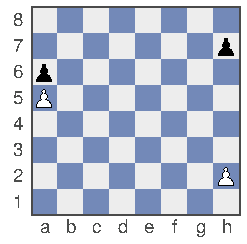
\includegraphics[width=\linewidth]{figures/two.pdf}
\caption{\pos{W~a5~h2 / B~a6~h7}: $2$}
\end{subfigure}\hfill
\begin{subfigure}[t]{0.16\textwidth}\centering
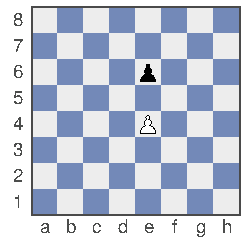
\includegraphics[width=\linewidth]{figures/star.pdf}
\caption{\pos{W~e4 / B~e6}: $\star$}
\end{subfigure}\hfill
\begin{subfigure}[t]{0.16\textwidth}\centering
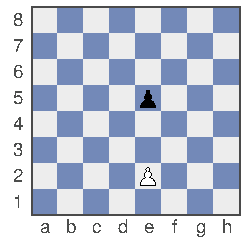
\includegraphics[width=\linewidth]{figures/up.pdf}
\caption{\pos{W~e2 / B~e5}: ${\uparrow}$}
\end{subfigure}\hfill
\begin{subfigure}[t]{0.16\textwidth}\centering
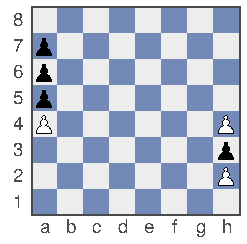
\includegraphics[width=\linewidth]{figures/tiny1_2025.pdf}
\caption{\pos{W~a4~h2~h4 / B~a5~a6~a7~h3}: $\tinyg{1}$}
\end{subfigure}
\caption{Pawn positions with the basic values (cylinder: files a and h adjacent). Each value holds in all nine
settings (Section~\ref{sec:ep}) except in (c), which is $2$ only with e.p.\ on and ${\Uparrow}\star$ with
e.p.\ off.}
\label{fig:basic}
\end{figure*}

\begin{definition}[E.p.-aware passed pawn]\label{def:epaware}
A pawn is \emph{passed} if it passes the textbook test \emph{and} cannot be captured en passant on the
opponent's next move.
\end{definition}

One more white pawn makes the difference decisive. In \pos{W~a2~b3 / B~b4} black has no move, and the textbook
test lets white win at once with a2--a4. Under Definition~\ref{def:epaware}, every white move lets black capture
on a3, directly or en passant, and win the race that follows under the count rule, so the value is $0$. Across
the census of Section~\ref{sec:atlas}, every position with at most six pawns on ordinary boards of width at
most four, the stricter test changes at least $18{,}137$ of the $231{,}071$ values (a few more changes are hidden
where both values exceed the display range), and $4{,}070$ of them in outcome \lab{C1}.

The three race rules and three e.p.\ options (textbook test, e.p.-aware test, e.p.\ off) give nine
\emph{settings}. Every value uses the \emph{default setting}, the count rule with the e.p.-aware test, unless
we say otherwise.

\subsection{Components and the Cut Lemma}
A pawn changes file only by capturing onto a file where an enemy pawn stands (en passant included), so an empty
file stays empty forever and the pawns on either side of it never interact. Each block of neighboring occupied
files is a game of its own, a \emph{component}, and a position is the sum of its components; on the cylinder a
component is an arc or one \emph{ring} that uses every file.

\begin{theorem}[Cut lemma; \lab{P}, \lab{C2}]\label{thm:cut}
A pawn position on $\cyl{n}$ with at least one empty file has the same value as the position on
$\flatb{n-1}$ obtained by cutting the cylinder open along that file.
\end{theorem}

\begin{proof}
No pawn can move onto the empty file, so cutting the board there changes no legal move, no en passant right and
no passed-pawn test: the files beside the cut lose only a neighbor that stays empty forever.
\end{proof}

Hence values only a cylinder can make must come from rings (Section~\ref{sec:atlas});
Section~\ref{sec:sums-hss} says when a sum of components still names the right winner.
